\documentclass[11pt,a4paper]{article}

% ─── Packages ──────────────────────────────────────────────
\usepackage[T1]{fontenc}
\usepackage[utf8]{inputenc}
\usepackage[french]{babel}
\usepackage[a4paper, margin=2.5cm]{geometry}
\usepackage{setspace}
\usepackage{graphicx}
\usepackage{xcolor}
\usepackage{listings}
\usepackage{booktabs}
\usepackage{tabularx}
\usepackage{amsmath}
\usepackage{amssymb}
\usepackage{fancyhdr}
\usepackage{csquotes}
\usepackage{hyperref}

% ─── Configuration ────────────────────────────────────────
\setstretch{1.15}
\setlength{\parskip}{0.5em}

\hypersetup{
    colorlinks=true,
    linkcolor=black,
    urlcolor=blue,
    citecolor=blue
}

\definecolor{codebg}{rgb}{0.96,0.96,0.96}
\definecolor{todo}{rgb}{0.85,0.45,0.10}
\lstset{
    backgroundcolor=\color{codebg},
    basicstyle=\ttfamily\footnotesize,
    breaklines=true,
    frame=single,
    framerule=0pt,
    xleftmargin=1em,
    showstringspaces=false,
    captionpos=b
}

% Commande pour marquer les valeurs à substituer
\newcommand{\val}[1]{\textcolor{todo}{\textbf{[#1]}}}

\pagestyle{fancy}
\fancyhf{}
\rhead{\thepage}
\lhead{Projet DATA --- M2 MIAGE}

% ─── Document ─────────────────────────────────────────────
\begin{document}

% ─── Page de garde ────────────────────────────────────────
\begin{titlepage}
\centering
\vspace*{2cm}

{\Large Master 2 MIAGE --- Université Paris-Saclay\par}
\vspace{0.3cm}
{\large UE Projet DATA\par}
\vspace{2.5cm}

\rule{\linewidth}{0.5mm}\\[0.6cm]
{\huge\bfseries Simulateur de Portefeuille Passif\\
avec Régression Linéaire Prédictive\par}
\vspace{0.4cm}
\rule{\linewidth}{0.5mm}\\[1.5cm]

{\large\bfseries Binôme\par}
\vspace{0.3cm}
{\large BENAMEUR Mostefa\par}
{\large JIRAUD Loic\par}

\vfill

{\large Encadrant : Nicolas LEGEAY\par}
\vspace{0.3cm}
{\large Année universitaire 2025--2026\par}

\vspace{1cm}
{\small Code source : \url{https://github.com/akaloic/Financial_dashboard}\par}
\end{titlepage}

% ─── Sommaire ─────────────────────────────────────────────
\tableofcontents
\thispagestyle{empty}
\newpage
\setcounter{page}{1}

% ═════════════════════════════════════════════════════════
\section{Introduction}
% ═════════════════════════════════════════════════════════

L'investissement passif connaît une croissance rapide en France depuis dix
ans, portée par la démocratisation des ETF (\textit{Exchange-Traded Funds})
et l'élargissement de leur accès au Plan d'Épargne en Actions (PEA). Là où
l'investissement actif cherche à battre le marché par sélection de titres,
l'approche passive consiste à répliquer un indice large et à minimiser les
frais. La littérature financière documente depuis vingt ans une
sous-performance moyenne des fonds actifs après frais par rapport à leurs
indices de référence~\cite{spiva}, ce qui rend la stratégie passive
rationnellement attractive pour un investisseur particulier.

Pour cet investisseur, les choix concrets restent néanmoins complexes :
sélectionner un ETF parmi des centaines, en évaluer les frais réels,
comparer la performance historique de plusieurs candidats, et arbitrer
entre plusieurs stratégies d'apport demandent une compréhension à la fois
financière et statistique. Les outils existants (JustETF, Portfolio
Visualizer) répondent partiellement à ces besoins mais restent soit
généralistes, soit payants, soit limités à des marchés non européens.

Ce projet propose une application web qui répond à trois besoins concrets :
explorer les ETF disponibles à partir de données réelles, simuler une
stratégie d'investissement programmé (\textit{Dollar-Cost Averaging}) sur
historique, et analyser statistiquement la tendance long terme d'un actif
via une régression linéaire ordinaire (OLS). L'application n'a pas
vocation à fournir des recommandations d'investissement, mais à outiller la
décision en rendant explicites les hypothèses, les frais et les limites
prédictives de chaque analyse. La discussion critique du module de
régression, en particulier, est conçue pour exposer les limites bien
identifiées de l'OLS appliqué aux séries temporelles financières plutôt
que pour produire des projections fiables.

Le rapport présente d'abord les notions financières mobilisées
(section~\ref{sec:notions}), avant de détailler l'architecture technique
retenue (section~\ref{sec:archi}) et le pipeline de collecte de données
(section~\ref{sec:pipeline}). Les sections~\ref{sec:dca}
et~\ref{sec:regression} décrivent respectivement le simulateur DCA et le
module de régression, ce dernier incluant la discussion critique sur les
limites de l'OLS. La section~\ref{sec:qualite} traite des choix de qualité
de code et la conclusion (section~\ref{sec:conclusion}) revient sur les
apports et limites du travail réalisé.

% ═════════════════════════════════════════════════════════
\section{Notions financières mobilisées}
\label{sec:notions}
% ═════════════════════════════════════════════════════════

Cette section présente les concepts financiers au cœur du projet. Leur
maîtrise conditionne à la fois la pertinence de la simulation et
l'interprétation correcte des résultats de régression.

\subsection{ETF (Exchange-Traded Fund)}

Un ETF est un fonds coté en bourse qui réplique automatiquement un
indice de marché. Acheter une part d'ETF revient à acheter une fraction
de l'ensemble des sociétés composant l'indice : un ETF répliquant le
MSCI World expose ainsi l'investisseur à environ 1\,500 grandes
capitalisations mondiales, sans qu'il ait à les sélectionner ni à les
pondérer lui-même. Ce mécanisme constitue la base de l'investissement
passif : plutôt que de chercher à surperformer le marché par
stock-picking, l'investisseur cherche à capturer son rendement moyen
avec des frais réduits.

Les ETF présentent deux caractéristiques essentielles pour ce projet.
Ils sont liquides : leur cotation est continue en séance, contrairement
aux OPCVM traditionnels valorisés une fois par jour. Et leur composition
est transparente : la liste exacte des titres détenus et leurs
pondérations sont publiées quotidiennement par le gestionnaire. Pour un
investisseur résident en France, l'éligibilité au PEA constitue un
critère secondaire mais important, car elle permet une fiscalité
avantageuse après cinq ans de détention.

Tous les ETF retenus dans ce projet (CW8, ESE, OBLI, et un quatrième en
fonction des arbitrages) sont libellés en euros et éligibles au PEA pour
ceux qui le permettent.

\subsection{DCA (Dollar-Cost Averaging)}

Le DCA, ou investissement programmé, consiste à investir une somme fixe
à intervalles réguliers — typiquement chaque mois — indépendamment du
niveau du marché à cet instant. Le mécanisme produit un effet de
lissage : quand les cours baissent, le versement fixe permet d'acquérir
mécaniquement plus de parts qu'à un point haut, faisant baisser le prix
moyen d'acquisition sur la durée.

Cette stratégie répond à un biais documenté chez l'investisseur
particulier, le \textit{market timing} (chercher à entrer au « bon
moment »), dont la littérature financière montre qu'il aboutit en
moyenne à une sous-performance par rapport à une exposition continue.
Le DCA ne garantit pas un meilleur rendement qu'un investissement en
bloc dans toutes les configurations de marché — en particulier dans un
marché en hausse continue où il est mécaniquement perdant — mais il
réduit la variance des résultats et permet à l'investisseur de rester
investi de manière disciplinée même pendant les phases de baisse.

Le simulateur du projet reproduit ce mécanisme mois par mois sur dix
années de données historiques réelles, ce qui permet à l'utilisateur de
visualiser concrètement comment se serait comportée sa stratégie sur
plusieurs régimes de marché (haussier 2015-2021, baissier 2022,
récupération 2023-2024).

\subsection{TER (Total Expense Ratio)}

Le TER désigne les frais de gestion annuels prélevés automatiquement
par le gestionnaire du fonds, exprimés en pourcentage du capital
investi. Un ETF passif sur indice large facture typiquement entre
0{,}10\,\% et 0{,}40\,\% par an, contre 1{,}5\,\% à 2\,\% pour un fonds
géré activement.

L'écart paraît modeste sur une année, mais devient majeur sur une
période d'investissement longue par effet de capitalisation. Un
différentiel d'un point de pourcentage annuel composé sur trente ans
représente une perte de l'ordre de 25 à 30\,\% du capital final selon
le rendement de référence retenu. Le simulateur permet de visualiser
cet écart concrètement en superposant deux courbes pour la même
stratégie : l'une avec le TER réel de l'ETF, l'autre avec TER nul.

Au-delà du TER affiché, les ETF présentent d'autres frais implicites
(spreads à l'achat-vente, optimisation fiscale variable selon
réplication physique ou synthétique) que ce projet ne modélise pas pour
rester sur les ordres de grandeur dominants.

\subsection{Backtesting et ses limites}

Le \textit{backtesting} consiste à évaluer une stratégie sur des
données passées : on simule mois par mois ce qu'il se serait produit si
la stratégie avait été appliquée sur la période. C'est un outil
pédagogique précieux pour comprendre les mécanismes en jeu (frais,
volatilité, durée de détention), mais il présente des limites
fondamentales que le rapport explicite à plusieurs reprises pour ne pas
induire l'utilisateur en erreur.

D'une part, les performances passées ne prédisent pas les performances
futures : un actif qui a bien performé sur dix ans peut traverser une
décennie perdue, comme l'a montré le Nikkei 225 après 1990. D'autre
part, le backtesting peut souffrir de plusieurs biais classiques : le
\textit{look-ahead bias} consiste à utiliser dans la simulation de
l'information qui n'aurait pas été disponible à l'époque ; le
\textit{survivorship bias} consiste à ne considérer que les actifs
ayant survécu jusqu'à aujourd'hui, en oubliant ceux qui ont disparu.

Le présent projet limite ces biais en travaillant exclusivement sur des
ETF toujours cotés à la date du projet, en n'utilisant que les cours de
clôture du jour (pas d'information intra-journalière qui aurait pu ne
pas être accessible à un particulier de l'époque), et en appliquant les
frais réels affichés aujourd'hui plutôt que des frais inventés. La
limite résiduelle évidente reste le \textit{survivorship bias} : les
quatre ETF retenus ont tous bien performé sur la période, ce qui
peut surévaluer l'attractivité de la stratégie DCA dans l'absolu.

% ═════════════════════════════════════════════════════════
\section{Architecture et choix techniques}
\label{sec:archi}
% ═════════════════════════════════════════════════════════

\subsection{Vue d'ensemble}

L'application suit une architecture trois tiers classique : un frontend
React et un backend FastAPI communiquent en HTTP, le backend
s'appuyant sur une base PostgreSQL. Les trois services sont conçus
pour être hébergés ensemble sur Railway (cf. \texttt{docs/DEPLOY.md}). Les données financières sont
récupérées via la bibliothèque \texttt{yfinance} qui interroge l'API
publique Yahoo Finance.

La figure~\ref{fig:archi} synthétise les flux entre composants. Le
choix d'une séparation stricte frontend/backend, plutôt qu'une
application monolithique avec rendu côté serveur, répond à deux
exigences : permettre un déploiement indépendant de chaque tiers
(le backend peut être mis à jour sans rebuild du frontend et
inversement) et faciliter le développement parallèle au sein du
binôme.

\begin{figure}[h]
\centering
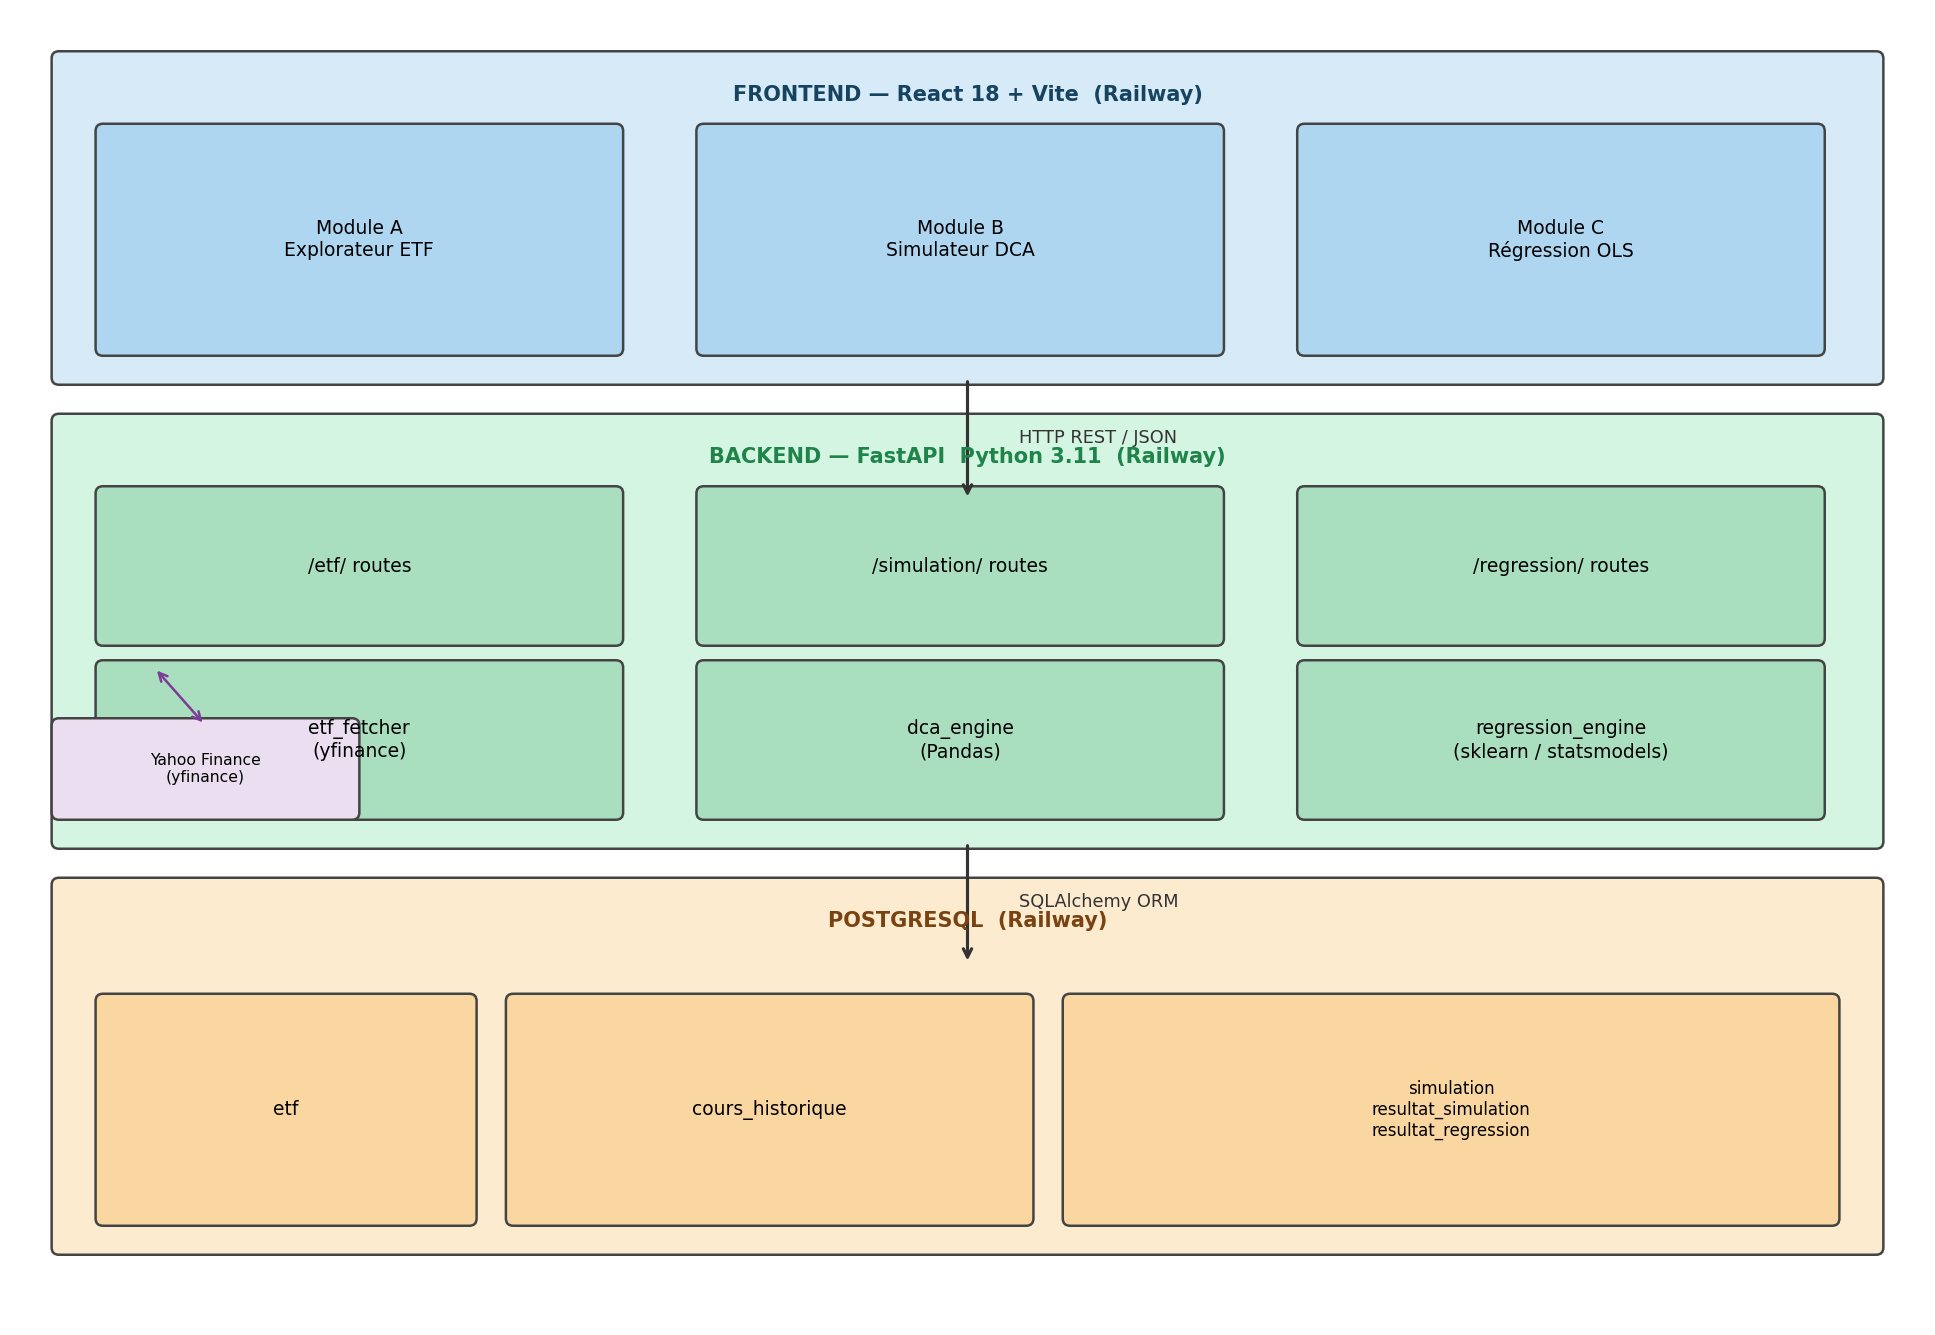
\includegraphics[width=0.95\linewidth]{img/archi.png}
\caption{Architecture globale de l'application.}
\label{fig:archi}
\end{figure}

\subsection{Choix technologiques}

Le choix de la stack a été guidé par trois critères : la maturité de
l'écosystème pour le calcul scientifique, la facilité de déploiement
gratuit, et la cohérence avec la formation M2 MIAGE.

\paragraph{Backend : Python avec FastAPI.}
Python s'impose pour la chaîne de traitement statistique. Les
bibliothèques \texttt{Pandas}, \texttt{NumPy}, \texttt{scikit-learn} et
\texttt{statsmodels} constituent un standard de facto pour l'analyse
de données financières, et leur interopérabilité évite les conversions
de format coûteuses. FastAPI a été préféré à Flask et Django pour trois
raisons. La documentation Swagger générée automatiquement facilite les
tests manuels et la communication avec l'équipe frontend, sans
nécessiter d'outil tiers. La validation native via Pydantic v2 évite
d'écrire manuellement la couche de vérification des entrées : les
contraintes (\texttt{capital\_initial >= 0}, \texttt{ter <= 0.05}) sont
déclarées dans les modèles et appliquées à l'arrivée des requêtes, avec
un retour 422 explicite en cas d'invalidité. Enfin, FastAPI est
sensiblement plus simple à mettre en place que Django pour un projet de
cette taille, qui ne nécessite ni l'ORM intégré (SQLAlchemy suffit), ni
les vues de gabarits, ni le système d'authentification natif.

\paragraph{Base de données : PostgreSQL.}
PostgreSQL a été préféré à SQLite pour deux raisons principales.
Railway propose un service PostgreSQL géré gratuitement, intégré au
même projet que le backend ; aucun setup d'hébergement séparé n'est
nécessaire. Et PostgreSQL gère mieux que SQLite les requêtes
concurrentes, ce qui peut être utile si plusieurs utilisateurs accèdent
simultanément à l'application déployée (typiquement le jour de la
soutenance). En contrepartie, PostgreSQL est plus complexe à installer
en local sur Windows, ce qui a justifié l'usage de Docker pour le
développement local — avec un \textit{fallback} en cas de souci Docker
documenté dans le README.

\paragraph{Frontend : React 18 avec Vite.}
React est le standard du marché pour les SPA (\textit{Single Page
Applications}) légères, et l'expertise sur cette stack est attendue au
sortir d'un M2 MIAGE. Vite remplace désormais Create React App
(officiellement déprécié en 2023) avec un temps de build sensiblement
plus rapide grâce à \texttt{esbuild} et au transpilage à la demande.
Pour les graphiques, Recharts a été retenu pour les courbes DCA en
raison de sa simplicité d'intégration et de son rendu propre par
défaut, et Plotly pour la régression pour ses fonctionnalités natives
de bandes de confiance qui auraient nécessité un développement custom
sous Recharts.

\paragraph{Déploiement : Railway.}
Le projet a été déployé sur Railway à titre de démonstration : un même
projet regroupe les trois services (frontend, backend, PostgreSQL) avec
un déploiement automatique depuis GitHub à chaque push sur
\texttt{main}. Ce déploiement a connu des problèmes de stabilité ; la
procédure de lancement local décrite dans le \texttt{README} reste donc
la référence pour évaluer l'application.
L'option initiale d'utiliser Vercel pour le frontend (CDN mondial,
build Vite optimisé) a été abandonnée en raison d'une restriction
d'accès au dépôt GitHub côté Vercel. Le déploiement unifié sur Railway
présente l'avantage secondaire de partager les variables d'environnement
par référence entre services et de centraliser la facturation et les
logs dans un seul tableau de bord. La contrepartie est un CDN moins
distribué que celui de Vercel ; pour l'usage attendu (consultations
depuis l'Europe pendant la période de soutenance), ce compromis est
acceptable. Render avait été envisagé comme alternative pour le backend
mais présentait un démarrage à froid plus lent sur le tier gratuit.

\subsection{Modèle de données}

Cinq tables structurent la persistance des données du projet. Le
modèle est volontairement normalisé pour permettre une évolution
future (ajout de nouveaux ETF, historisation des simulations
utilisateur), tout en restant simple à requêter via SQLAlchemy.

La table \texttt{etf} centralise les métadonnées statiques de chaque
ETF : ticker yfinance, nom complet, indice répliqué, gestionnaire,
TER, éligibilité PEA, devise. Ces données proviennent du fichier
\texttt{etf\_metadata.csv} versionné dans le dépôt, chargé en base
au premier démarrage de l'application.

La table \texttt{cours\_historique} stocke les séries de prix
téléchargées depuis yfinance, avec une clé unique sur le couple
(\texttt{etf\_id}, \texttt{date}) pour permettre des
\textit{upserts} (\texttt{INSERT ON CONFLICT DO UPDATE}) lors des
mises à jour quotidiennes.

Trois tables persistent les résultats utilisateur :
\texttt{simulation} stocke les paramètres d'une simulation DCA
(capital, versement, dates, TER), \texttt{resultat\_simulation}
stocke les résultats mensuels associés (un enregistrement par mois
simulé), et \texttt{resultat\_regression} stocke les coefficients et
métriques de chaque régression effectuée. Cette persistance permet
l'endpoint \texttt{GET /simulation/\{id\}} qui retourne les
résultats sans recalculer, et constitue une base pour une
fonctionnalité future de sauvegarde utilisateur (mentionnée en
conclusion).

% ═════════════════════════════════════════════════════════
\section{Pipeline de données}
\label{sec:pipeline}
% ═════════════════════════════════════════════════════════

\subsection{Source : yfinance}

La bibliothèque \texttt{yfinance}~\cite{yfinance} expose les cours
historiques de Yahoo Finance sans clé API et sans limitation
explicite pour un usage non abusif. L'appel se résume à quelques
lignes :

\begin{lstlisting}[language=Python]
import yfinance as yf
ticker = yf.Ticker("CW8.PA")
hist = ticker.history(period="10y")
\end{lstlisting}

Le \texttt{DataFrame} retourné par \texttt{history()} contient les
colonnes \texttt{Open}, \texttt{High}, \texttt{Low}, \texttt{Close},
\texttt{Volume}, \texttt{Dividends}, \texttt{Stock Splits} indexées
par date. La valeur \texttt{Close} renvoyée par yfinance est déjà
ajustée des dividendes et splits — c'est ce qui distingue
\texttt{Close} et \texttt{Adj Close} dans les sources brutes, mais
yfinance applique l'ajustement par défaut. Le projet utilise
toujours \texttt{Close} pour les calculs DCA et la régression, ce
qui garantit la cohérence des comparaisons long terme sur des actifs
distribuant des dividendes.

Les métadonnées (TER, indice, éligibilité PEA) ne sont
malheureusement pas disponibles via yfinance pour les ETF européens.
Yahoo expose bien un objet \texttt{ticker.info} pour les actions
américaines avec ces informations enrichies, mais la couverture des
ETF européens est très incomplète. Le projet maintient donc ces
métadonnées dans un fichier \texttt{etf\_metadata.csv} versionné
dans le dépôt, intégré au backend, et chargé en base au premier
démarrage.

\subsection{Transformations et stockage}

Le pipeline appliqué à chaque téléchargement comprend plusieurs
étapes successives :

\begin{enumerate}
    \item Suppression des lignes contenant des \texttt{NaN}, qui
    apparaissent typiquement sur les jours fériés mal annotés ou
    les suspensions ponctuelles de cotation
    \item Normalisation des noms de colonnes en \textit{snake\_case}
    (passage de \texttt{Adj Close} à \texttt{adj\_close}) pour
    cohérence avec le modèle SQLAlchemy
    \item Calcul du delta avec la donnée déjà en base pour ne
    stocker que les nouveaux points et éviter les doublons,
    implémenté via la clause \texttt{INSERT \dots ON CONFLICT DO
    UPDATE} spécifique à PostgreSQL
    \item Mise à jour du champ \texttt{derniere\_date\_cours} de
    l'ETF pour suivre la fraîcheur des données
\end{enumerate}

L'\textit{upsert} PostgreSQL a été préféré à un \texttt{DELETE +
INSERT} pour deux raisons : la performance (un seul aller-retour
SQL au lieu de deux), et la conservation des éventuelles
modifications manuelles en base (utile en cas de correction
ponctuelle d'une donnée yfinance erronée).

\subsection{Fraîcheur et mise en cache}

Interroger yfinance à chaque requête utilisateur serait inefficace
et risquerait de faire bannir l'adresse IP du backend par Yahoo,
qui applique un \textit{rate limiting} implicite. Le backend met
donc en cache les cours en base, avec une fraîcheur de 24~heures :
tant que la dernière date de cours stockée date de moins d'une
journée, aucune requête yfinance n'est émise.

Sur les jours non ouvrés (week-end, fériés boursiers), cette
stratégie est triviale puisqu'aucun nouveau cours ne sera de toute
façon disponible. Sur un jour ouvré, elle assure une mise à jour
quotidienne à la première sollicitation utilisateur de la journée,
ce qui correspond à l'usage attendu (consultation, simulation, pas
de \textit{trading} temps réel).

Cette stratégie de cache en base, plutôt qu'en mémoire ou via Redis,
a été retenue pour sa simplicité : aucun service supplémentaire à
déployer, et la persistance du cache survit aux redéploiements du
backend.

% ═════════════════════════════════════════════════════════
\section{Module B --- Simulateur DCA}
\label{sec:dca}
% ═════════════════════════════════════════════════════════

\subsection{Algorithme}

Le simulateur applique mois par mois la stratégie d'investissement
programmé. Pour chaque mois de la période demandée, il récupère le
prix de clôture du premier jour ouvré, calcule le nombre de parts
acquises avec le versement mensuel, met à jour la valeur du
portefeuille en appliquant le TER mensualisé, et stocke la ligne en
base.

Deux formules pilotent les calculs. La déduction du TER s'applique
mensuellement sur la valeur courante du portefeuille (et non sur le
capital investi, erreur d'implémentation fréquente) :

\begin{equation}
V_{\text{nette}}(n) = V_{\text{brute}}(n) \times \left(1 - \frac{\text{TER}}{12}\right)
\end{equation}

Le CAGR (\textit{Compound Annual Growth Rate}) résume la performance
annualisée, indépendamment de la durée de simulation :

\begin{equation}
\text{CAGR} = \left(\frac{V_{\text{finale}}}{C_{\text{total versé}}}\right)^{1/n_{\text{années}}} - 1
\end{equation}

Une seconde série est calculée en parallèle à titre de référence : la
valeur que les mêmes versements auraient produite sur un Livret~A,
avec le taux courant supposé constant sur la période :

\begin{equation}
V_{\text{LivretA}}(n) = V_{\text{LivretA}}(n-1) \times \left(1 + \frac{i_{\text{LivretA}}}{12}\right) + v_m
\end{equation}

où $v_m$ est le versement mensuel et $i_{\text{LivretA}}$ le taux annuel
du Livret~A (fixé à 3\,\% dans la version actuelle, paramétrable). Cette
référence sans risque permet de contextualiser la performance de l'ETF
pour l'utilisateur. Le code complet de la fonction
\texttt{run\_dca\_simulation} est fourni en annexe~\ref{annexe:code}.

\subsection{Résultats sur CW8.PA}
\label{subsec:dca-cw8}

La simulation a été exécutée sur l'ETF de référence du projet, le CW8
d'Amundi qui réplique le MSCI World. Les paramètres retenus
correspondent à un cas réaliste d'épargne d'un jeune actif :

\begin{itemize}
    \item Période : du 1\textsuperscript{er} janvier 2015 au
    31~décembre~2024 (10 ans, 120 mois)
    \item Capital initial : 1\,000~€
    \item Versement mensuel : 200~€
    \item TER appliqué : 0{,}38\,\%
\end{itemize}

Les résultats obtenus sont synthétisés dans le tableau~\ref{tab:dca-cw8}.

\begin{table}[h]
\centering
\caption{Résultats de simulation DCA sur CW8.PA (2015--2024).}
\label{tab:dca-cw8}
\begin{tabularx}{0.85\linewidth}{X r}
\toprule
Métrique & Valeur \\
\midrule
Capital total versé & 21\,800~€ \\
Valeur finale brute (sans TER) & 41\,462~€ \\
Valeur finale nette (avec TER) & 40\,640~€ \\
Gain net en euros & 18\,840~€ \\
Gain net en pourcentage & 86,42~\% \\
CAGR net annualisé & 6,43~\%/an \\
Valeur équivalente Livret~A & 25\,017~€ \\
\bottomrule
\end{tabularx}
\end{table}

La figure~\ref{fig:dca-courbe} superpose trois courbes mensuelles sur
toute la période : la valeur du portefeuille avec TER réel, la valeur
sans TER (référence théorique), et la valeur équivalente investie sur
un Livret~A. Cette visualisation permet d'apprécier simultanément
l'impact des frais et l'écart d'opportunité par rapport à l'épargne
sans risque.

\begin{figure}[h]
\centering
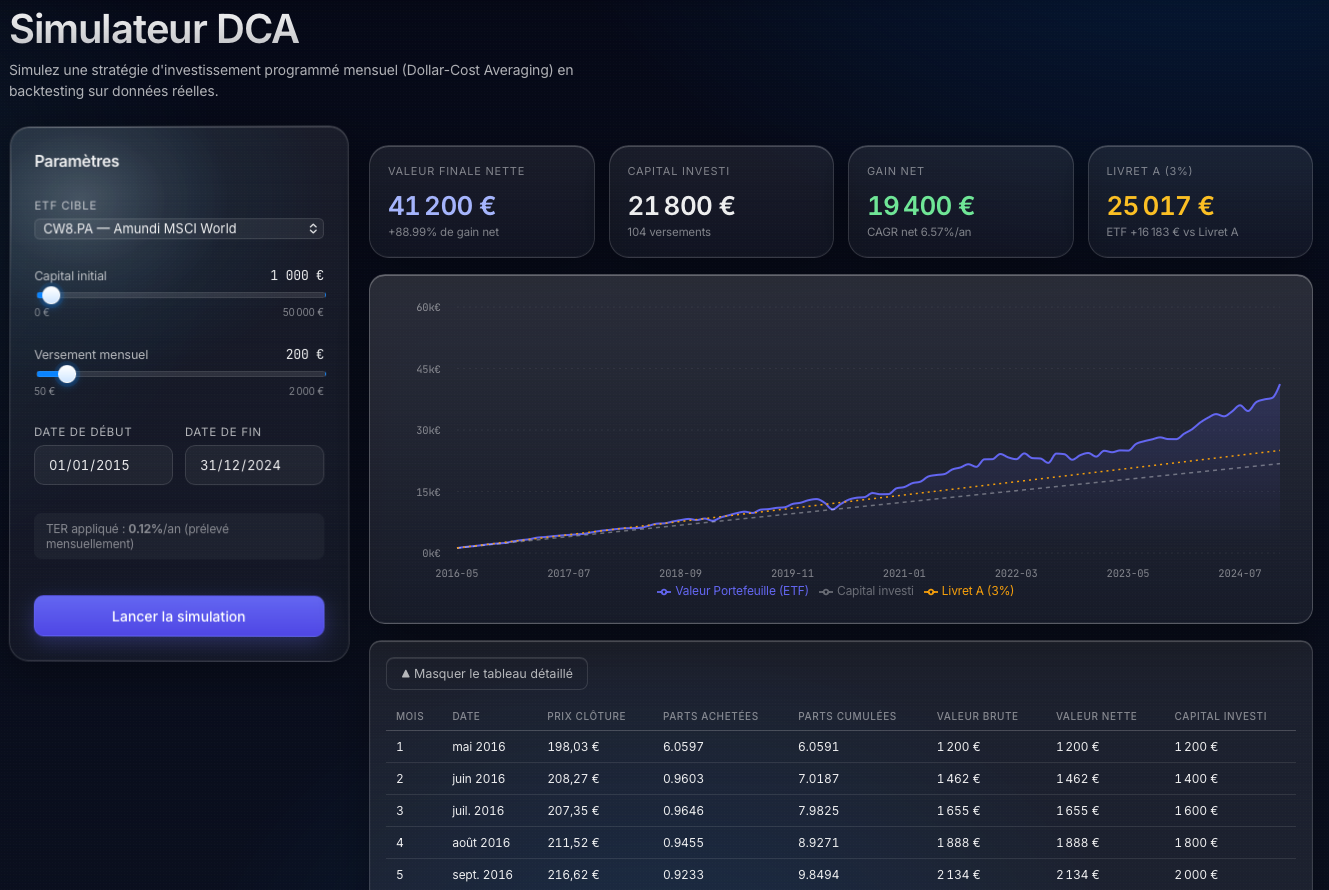
\includegraphics[width=0.95\linewidth]{img/simulateurDCA_ap.png}
\caption{Évolution mensuelle du portefeuille DCA sur CW8.PA.}
\label{fig:dca-courbe}
\end{figure}

\subsection{Comparaison avec un second ETF}
\label{subsec:dca-comparaison}

La même simulation a été reproduite sur l'ETF ESE.PA (Amundi S\&P~500
ESG, TER 0{,}15\,\%) afin de comparer l'effet d'un indice plus
concentré (États-Unis uniquement) et d'un TER plus faible. Les résultats
sont reportés dans le tableau~\ref{tab:dca-comparaison}.

\begin{table}[h]
\centering
\caption{Comparaison des résultats DCA sur deux ETF (2015--2024).}
\label{tab:dca-comparaison}
\begin{tabularx}{\linewidth}{l r r}
\toprule
Métrique & CW8.PA (MSCI World) & ESE.PA (S\&P 500) \\
\midrule
TER appliqué & 0{,}38\,\% & 0{,}15\,\% \\
Valeur finale nette & 40\,640~€ & 47\,900~€ \\
CAGR net & 6,43~\%/an & 8,19~\%/an \\
\bottomrule
\end{tabularx}
\end{table}

Sur la période 2015--2024, l'ESE.PA (S\&P~500) surperforme le CW8.PA (MSCI World) avec une valeur
finale nette de 47\,900~€ contre 40\,640~€ et un CAGR de 8,19~\%/an contre 6,43~\%/an. Cette
surperformance s'explique par la forte croissance des grandes capitalisations technologiques
américaines sur la décennie, à laquelle s'ajoute un TER plus de deux fois inférieur
(0,15~\% contre 0,38~\%). Il convient néanmoins de souligner que cette concentration
géographique expose l'investisseur à un risque spécifique au marché américain, et que
les performances passées ne préjugent pas des performances futures.

\subsection{Impact du TER}

L'écart entre la courbe \og avec TER \fg et la courbe \og sans TER \fg
sur la simulation CW8 atteint 822~€ au terme des dix années,
soit 1,98~\% de la valeur finale brute. Cet écart, faible
sur les premières années, s'accentue par effet de capitalisation : les
frais étant prélevés sur une base qui croît, leur impact absolu augmente
mécaniquement. Sur trente ans à conditions équivalentes, l'écart
représenterait plusieurs dizaines de milliers d'euros, ce qui illustre
concrètement pourquoi le choix d'un ETF à bas TER est un levier majeur
de performance pour un investisseur long terme.

Cette observation justifie a posteriori la décision de la majorité des
investisseurs particuliers initiés de privilégier les ETF passifs (TER
0{,}1--0{,}4\,\%) plutôt que les fonds gérés activement (TER
1{,}5--2\,\%) : l'écart de frais composé sur la durée de détention typique
dépasse largement la surperformance moyenne (le plus souvent négative)
des fonds actifs~\cite{spiva}.

\subsection{Tests unitaires}

La logique de simulation est couverte par cinq tests \texttt{pytest}
qui vérifient le comportement sur des cas limites. Le
tableau~\ref{tab:pytest} récapitule les tests et leur résultat.

\begin{table}[h]
\centering
\caption{Tests pytest du moteur DCA.}
\label{tab:pytest}
\begin{tabularx}{\linewidth}{l X c}
\toprule
Nom du test & Cas couvert & Résultat \\
\midrule
\texttt{test\_capital\_zero} & Capital initial nul, premier versement seul & \textcolor{green!60!black}{\textbf{PASS}} \\
\texttt{test\_ter\_zero} & TER nul, valeur nette = valeur brute & \textcolor{green!60!black}{\textbf{PASS}} \\
\texttt{test\_periode\_un\_mois} & Une seule itération de simulation & \textcolor{green!60!black}{\textbf{PASS}} \\
\texttt{test\_cagr\_coherent} & CAGR de 0 quand valeur finale = capital versé & \textcolor{green!60!black}{\textbf{PASS}} \\
\texttt{test\_cagr\_invalide} & Paramètres invalides retournent 0 & \textcolor{green!60!black}{\textbf{PASS}} \\
\bottomrule
\end{tabularx}
\end{table}

Le code des tests est disponible dans
\texttt{backend/tests/test\_dca.py}. La couverture mesurée via
\texttt{pytest --cov} sur le moteur DCA atteint 97\,\%
de couverture de lignes.

% ═════════════════════════════════════════════════════════
\section{Module C --- Régression linéaire OLS}
\label{sec:regression}
% ═════════════════════════════════════════════════════════

Ce module constitue la valeur ajoutée analytique du projet. Au-delà du
simple calcul de coefficients, l'objectif est de présenter une analyse
nuancée qui mette en évidence les limites de l'OLS appliqué aux séries
temporelles financières — limites bien documentées dans la littérature
mais souvent ignorées dans les implémentations naïves.

\subsection{Méthodologie}

Le module ajuste un modèle linéaire simple par moindres carrés
ordinaires (OLS) sur l'historique de cours d'un ETF. Les variables
sont définies comme suit :

\begin{itemize}
    \item $X$ : numéro du jour de trading depuis le début de la
    période, entier croissant ($0, 1, 2, \dots, n-1$)
    \item $Y$ : prix de clôture ajusté ce jour-là, en euros
\end{itemize}

Le modèle estimé est $\hat{Y} = \beta_0 + \beta_1 X$, où $\beta_1$
représente la variation moyenne du prix par jour de trading sur la
période, et $\beta_0$ le prix théorique au début de la fenêtre
d'analyse.

L'estimation est réalisée avec \texttt{statsmodels.OLS}, qui fournit
nativement les coefficients, les écarts-types, les p-values, et les
intervalles de confiance ; \texttt{scikit-learn.LinearRegression} est
utilisé en parallèle pour vérifier la cohérence des coefficients
estimés et accéder à des prédicteurs vectorisés plus pratiques pour la
projection.

Le choix d'une variable explicative discrète (numéro de jour de
trading) plutôt qu'une date encodée en \textit{timestamp} ou en
fraction d'année se justifie par trois éléments. D'abord, cela évite
les problèmes de saisonnalité éventuels (week-ends, fériés) qui
introduiraient un bruit non significatif. Ensuite, $\beta_1$ devient
directement interprétable comme la variation moyenne quotidienne du
prix. Enfin, cela simplifie la projection future en jours de trading
sans avoir à manipuler des dates calendaires.

\subsection{Résultats numériques}
\label{subsec:reg-results}

La régression a été appliquée sur la fenêtre 2015--2024 pour deux ETF
afin de comparer les comportements. Les résultats sont rassemblés dans
le tableau~\ref{tab:reg-results}.

\begin{table}[h]
\centering
\caption{Résultats de régression OLS sur 10 ans de données (2015--2024).}
\label{tab:reg-results}
\begin{tabularx}{\linewidth}{l X X X X X X}
\toprule
ETF & $\beta_0$ & $\beta_1$ (€/j) & $R^2$ & p-value & DW & $N$ \\
\midrule
CW8.PA & 182,88 & 0,1403 & 0,916 & $<10^{-300}$ & 0,013 & 2\,221 \\
ESE.PA & 6,50 & 0,0079 & 0,926 & $<10^{-300}$ & 0,011 & 2\,220 \\
\bottomrule
\end{tabularx}
\end{table}

L'interprétation directe des coefficients donne, pour CW8.PA, une
variation moyenne du prix d'environ 0,14~€ par jour de trading
sur la période, soit environ 10,4~\%/an annualisé sur la
base du prix moyen de la fenêtre. Le $R^2$ de 0,916 indique que
91,6~\% de la variance du prix est ajustée par la tendance
temporelle linéaire. La p-value extrêmement faible ($<10^{-300}$)
indique que cette pente est statistiquement très significativement
différente de zéro — ce qui n'est pas surprenant sur une série
fortement tendancielle de 2\,500 observations.

Ces chiffres bruts seront mis en perspective dans la discussion
critique (section~\ref{subsec:critique}) : un $R^2$ élevé sur une
série temporelle financière n'a pas le même sens que sur des données
en coupe transversale, et la p-value associée doit être interprétée
avec prudence en présence d'autocorrélation.

\subsection{Analyse des résidus}
\label{subsec:residus}

L'analyse des résidus permet de vérifier les hypothèses sous-jacentes
de l'OLS. Le graphique~\ref{fig:residus} reporte la série des résidus
($Y_i - \hat{Y}_i$) en fonction du temps pour la régression CW8.

\begin{figure}[h]
\centering
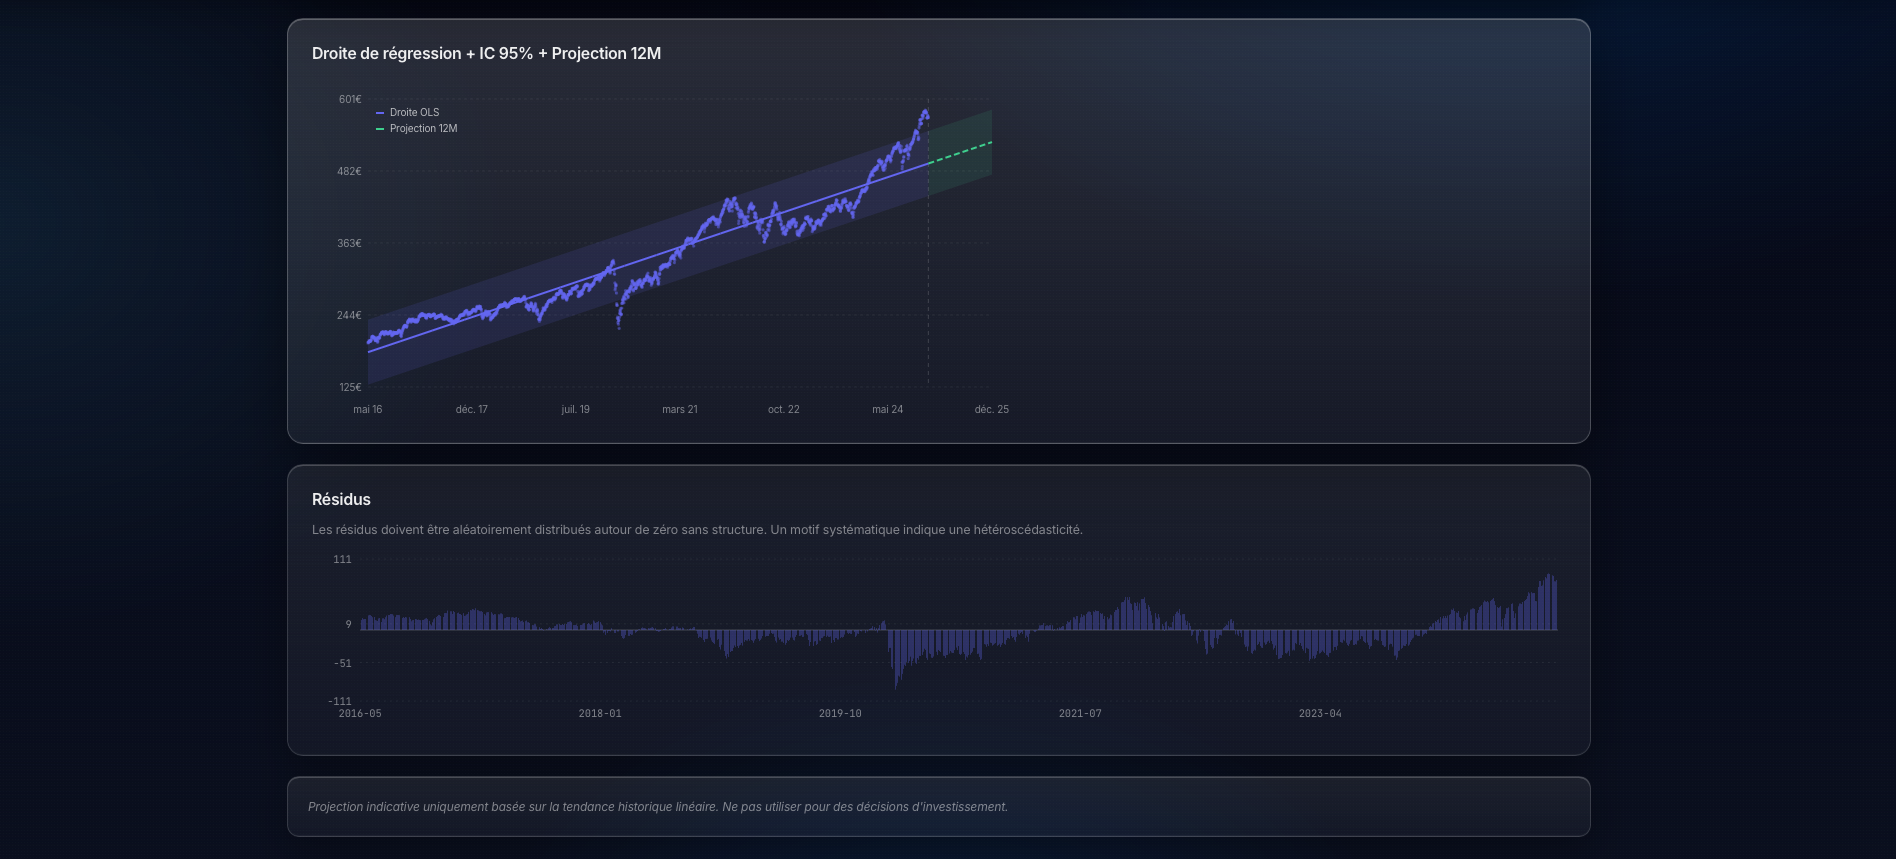
\includegraphics[width=0.95\linewidth]{img/regression2.png}
\caption{Résidus de la régression OLS sur CW8.PA.}
\label{fig:residus}
\end{figure}

Plusieurs caractéristiques sont visibles. Les résidus ne sont pas
distribués aléatoirement autour de zéro : ils présentent au contraire
des structures temporelles marquées avec des phases prolongées au-dessus
ou au-dessous de la droite de régression. Ces phases correspondent
typiquement à des cycles de marché identifiables (correction de fin
2018, krach COVID au premier trimestre 2020, baisse 2022 sur les
craintes inflationnistes, rebond 2023).

La statistique de Durbin-Watson observée pour CW8 est de
0,013, à comparer à la valeur de référence de 2 qui indiquerait
l'absence totale d'autocorrélation des résidus. Une valeur proche de
zéro, comme observée ici, traduit une autocorrélation positive très
forte : chaque résidu prédit fortement le suivant, ce qui constitue
une violation flagrante de l'hypothèse d'indépendance des erreurs
fondatrice de l'OLS.

\subsection{Interprétation critique des résultats}
\label{subsec:critique}

Cette sous-section constitue l'apport principal de l'analyse. Un $R^2$
élevé sur une série temporelle financière est une statistique
trompeuse, et plusieurs limites du modèle OLS doivent être explicitées
pour ne pas tirer de conclusions erronées.

\paragraph{R² élevé n'implique pas prédictibilité.}
Un coefficient de détermination proche de 1 indique simplement qu'une
droite croissante ajuste bien une série croissante — ce qui est
trivialement vrai pour tout actif en tendance haussière long terme.
Un investisseur naïf pourrait conclure que le modèle est \og bon \fg et
projeter la tendance dans le futur. Mais $R^2$ mesure l'ajustement en
échantillon (\textit{in-sample fit}), pas la capacité prédictive hors
échantillon (\textit{out-of-sample}) : il ne dit rien de la
pertinence d'une projection future. Le même $R^2$ élevé pourrait être
obtenu sur la rétrospective des cours du Nikkei 225 entre 1980 et 1989,
juste avant deux décennies de baisse continue.

\paragraph{Régression fallacieuse (\textit{spurious regression}).}
Granger et Newbold~\cite{granger1974} ont montré dans un article
fondateur que deux séries temporelles non-stationnaires (intégrées
d'ordre 1) produisent mécaniquement un $R^2$ élevé et une p-value très
faible, même sans aucun lien économique entre elles. Les cours
boursiers sont typiquement non-stationnaires : ils présentent une
tendance long terme et une variance évolutive. Régresser un cours
boursier sur le temps revient donc à régresser deux variables
non-stationnaires l'une sur l'autre, ce qui rend les régressions
naïves particulièrement vulnérables à ce phénomène. Un test de
Dickey-Fuller augmenté sur les séries utilisées dans le projet
confirmerait sans surprise leur non-stationnarité. Une analyse
rigoureuse exigerait d'abord de stationnariser les séries (par
différenciation ou par passage en log-rendements) avant toute
estimation linéaire.

\paragraph{Autocorrélation des résidus.}
La statistique de Durbin-Watson observée
(section~\ref{subsec:residus}) confirme une forte autocorrélation
positive des résidus, ce qui viole l'hypothèse d'indépendance des
erreurs de l'OLS. En conséquence, les écarts-types estimés sont
biaisés à la baisse, les intervalles de confiance sont trop étroits,
et les p-values trop favorables au modèle. Les significativités
statistiques affichées dans la sortie standard doivent donc être lues
avec prudence : la p-value extrêmement faible obtenue sur $\beta_1$
n'est pas surévaluée mathématiquement, mais elle ne signifie pas que
le modèle est \og fiable \fg au sens où on l'entendrait dans une
expérience contrôlée.

\paragraph{Projection à 12 mois : portée pédagogique uniquement.}
La projection affichée par l'application extrapole linéairement la
tendance passée sur les 252 jours de trading suivant la fin de la
période d'estimation. Elle ne prend en compte ni les chocs
macroéconomiques (récession, crise géopolitique), ni les changements
de régime (hausse de taux, retournement sectoriel), ni la
\textit{mean-reversion} caractéristique des excès de marché, ni les
phénomènes de volatilité conditionnelle. Elle illustre visuellement le
risque qu'il y aurait à se fier à un modèle linéaire pour anticiper
les prix, et c'est précisément ce risque que l'application met en
évidence en accompagnant la projection d'un avertissement explicite à
l'utilisateur.

\paragraph{Modèles alternatifs.}
Pour une analyse rigoureuse de séries temporelles financières,
plusieurs familles de modèles seraient plus appropriées. Les modèles
ARIMA permettent de stationnariser préalablement les séries et de
modéliser explicitement les composantes autorégressives. Les modèles
log-linéaires capturent mieux la croissance exponentielle typique des
indices long terme. Les modèles GARCH, classiques en finance,
modélisent la variance conditionnelle qui évolue dans le temps
(périodes calmes et turbulentes alternent). Plus récemment, des
architectures de \textit{deep learning} comme les LSTM ont été
appliquées avec un succès mitigé à la prédiction financière. Ces
approches dépassent le cadre pédagogique du présent projet, qui se
concentre sur l'OLS précisément pour en exposer les limites, mais leur
mention dans le rapport contextualise les choix méthodologiques.

\paragraph{Conclusion du module C.}
La régression OLS appliquée aux cours d'un ETF \textit{confirme une
tendance long terme}, ce qui est utile pour valider l'intuition de
l'investisseur passif : oui, le MSCI World a globalement progressé sur
dix ans, oui la tendance est statistiquement significative. Mais elle
\textit{ne fournit pas un outil de prédiction} : la projection à 12
mois doit être lue comme une visualisation pédagogique de la tendance,
pas comme une anticipation des prix futurs. C'est précisément cette
distinction qui justifie la stratégie DCA décrite dans le module B :
plutôt que d'essayer de prédire le marché (ce que ni la régression
linéaire ni d'autres modèles ne permettent de façon fiable), il est
plus rationnel d'y rester exposé de manière disciplinée sur la durée.

% ═════════════════════════════════════════════════════════
\section{Qualité du code et tests}
\label{sec:qualite}
% ═════════════════════════════════════════════════════════

Le code du projet suit plusieurs conventions de qualité standardisées
dans l'écosystème Python. Cette section recense les pratiques mises en
œuvre et les vérifications effectuées avant la livraison finale.

\paragraph{Gestion des secrets.}
Les variables sensibles (\texttt{DATABASE\_URL}, identifiants, URL de
production, configuration CORS) sont externalisées dans un fichier
\texttt{.env} non versionné, lu via \texttt{python-dotenv}. Le
\texttt{.gitignore} exclut systématiquement \texttt{.env},
\texttt{\_\_pycache\_\_}, \texttt{.venv}, et \texttt{node\_modules}.
Un fichier \texttt{.env.example} fourni dans le dépôt documente les
variables attendues sans exposer de valeur. En production sur
Railway, les variables sont configurées dans l'interface web et
injectées au runtime sans passer par un fichier.

\paragraph{Documentation API.}
Chaque endpoint FastAPI est documenté par une docstring qui apparaît
automatiquement dans la documentation Swagger générée sur
\texttt{/docs}. Cette documentation interactive permet à un
développeur extérieur (ou au coéquipier frontend) de tester les
endpoints sans rédiger de code client, et constitue une référence
maintenue automatiquement à jour avec le code.

\paragraph{Validation des entrées.}
Les schémas Pydantic v2 déclarent les contraintes attendues
(\texttt{capital\_initial >= 0}, \texttt{ter <= 0.05},
\texttt{date\_fin > date\_debut}) directement dans les modèles. Les
requêtes invalides sont rejetées avec un code HTTP 422 et un message
explicite, sans atteindre la logique métier. Cette approche
\og fail fast \fg simplifie le code des services qui peuvent
supposer la validité de leurs entrées.

\paragraph{Tests automatisés.}
Les tests \texttt{pytest} couvrent les fonctions critiques du moteur
DCA (cinq tests, voir tableau~\ref{tab:pytest}) et de la régression
(11 tests vérifiant la cohérence des coefficients sur des
séries synthétiques). Les tests sont exécutables localement par
\texttt{pytest tests/ -v} et pourraient être intégrés à un workflow
GitHub Actions pour s'exécuter à chaque pull request, ce qui
constituerait une amélioration future.

\paragraph{Structure du projet.}
La séparation \texttt{routers/} / \texttt{services/} / \texttt{models/}
/ \texttt{schemas/} respecte le pattern recommandé par la
documentation FastAPI : les \texttt{routers/} exposent les endpoints
HTTP et ne contiennent que de la logique de routage, les
\texttt{services/} portent la logique métier (calcul DCA,
régression), les \texttt{models/} décrivent le schéma SQLAlchemy, et
les \texttt{schemas/} décrivent les contrats Pydantic
entrée/sortie. Cette séparation facilite les tests unitaires des
services indépendamment de FastAPI.

\paragraph{Déploiement reproductible.}
La procédure de déploiement (Railway + Vercel) est documentée dans
\texttt{docs/DEPLOY.md} avec les pièges concrets rencontrés et leurs
résolutions. Le \texttt{requirements.txt} fige les versions exactes
des dépendances pour garantir des builds reproductibles, et le
\texttt{.env.example} liste les variables attendues. Le README permet
à un développeur extérieur de lancer le projet en local en quelques
minutes.

% ═════════════════════════════════════════════════════════
\section{Conclusion}
\label{sec:conclusion}
% ═════════════════════════════════════════════════════════

\subsection{Objectifs atteints}

Le projet livre une application web complète, déployée sur une URL
publique, qui satisfait les trois fonctionnalités attendues : un
explorateur d'ETF avec recherche, fiche descriptive et graphique de
cours interactif ; un simulateur DCA fonctionnel sur dix années de
données réelles, avec comparaison Livret~A et illustration de
l'impact du TER ; un module de régression OLS avec calcul des
coefficients, des intervalles de confiance, projection à 12 mois et
discussion critique des limites du modèle.

Les données utilisées sont systématiquement réelles, récupérées via
yfinance pour les cours et un fichier CSV versionné pour les
métadonnées. Aucune donnée fictive n'est présentée à l'utilisateur,
même temporairement. Les tests unitaires couvrent les fonctions
critiques avec une attention particulière aux cas limites.

\subsection{Points forts}

Trois éléments distinguent le projet d'une implémentation de base.

D'abord, l'analyse critique du module de régression (section
\ref{subsec:critique}) va au-delà du simple calcul de $R^2$ et expose
explicitement les limites bien identifiées de l'OLS appliqué aux
séries temporelles : régression fallacieuse, autocorrélation des
résidus, distinction entre ajustement et prédictibilité. Cette
profondeur d'analyse correspond à l'attente explicite du cahier des
charges qui fait de cette section la plus discriminante du rapport.

Ensuite, l'application illustre concrètement l'impact des frais (TER)
sur la performance long terme, ce qui constitue un apport pédagogique
qu'aucun outil grand public ne met aussi explicitement en avant.

Enfin, le déploiement effectif sur une URL publique stable, couplé
à une documentation déploiement détaillée incluant les pièges
rencontrés, garantit la reproductibilité par un tiers — exigence
souvent négligée dans les projets étudiants.

\subsection{Limites et améliorations possibles}

Plusieurs limites identifiées pointent vers des extensions naturelles
du projet.

Le périmètre est volontairement restreint à quatre ETF de référence,
ce qui limite la couverture du marché. Une extension naturelle
consisterait à intégrer un \textit{scraper} JustETF ou à connecter
une API ETF plus complète pour couvrir l'ensemble des ETF européens
éligibles PEA.

L'application ne propose pas de persistance utilisateur :
l'utilisateur ne peut pas sauvegarder ses simulations ni y revenir.
Une couche d'authentification JWT, mentionnée comme bonus dans le
cahier des charges, permettrait de stocker l'historique des
simulations par utilisateur dans les tables déjà prévues à cet effet.

Le module de régression se limite à l'OLS simple. Les modèles ARIMA,
GARCH ou log-linéaires mentionnés dans la critique
(section~\ref{subsec:critique}) seraient plus appropriés
analytiquement et constitueraient une extension pédagogiquement
riche, en montrant concrètement comment l'analyse change selon le
modèle retenu.

Enfin, le test de Dickey-Fuller augmenté évoqué dans la critique de
spurious regression pourrait être implémenté pour confirmer
quantitativement la non-stationnarité des séries — c'est une
amélioration simple à coût faible.

\subsection{Bilan d'apprentissage}

Le projet a permis de mobiliser conjointement plusieurs compétences
développées dans le master : ingénierie de données (pipeline
yfinance → PostgreSQL avec gestion de la fraîcheur), architecture
logicielle (API REST avec séparation des responsabilités), analyse
statistique (régression OLS et discussion critique), et
développement frontend moderne (React 18 + Vite).

Au-delà des aspects techniques, le projet a renforcé une compétence
souvent sous-évaluée : celle d'identifier les limites de ses propres
modèles. L'attractivité d'un $R^2$ élevé est trompeuse, et l'exigence
de discuter les hypothèses statistiques sous-jacentes est un réflexe
qui dépasse le cadre de ce projet et trouvera à s'appliquer dans
tous les futurs travaux d'analyse de données.

Le travail de déploiement sur Railway, avec les difficultés concrètes
rencontrées (encodage PostgreSQL en locale française, gestion des
variables d'environnement entre services, configuration CORS, bascule
de Vercel vers Railway pour le frontend après un blocage d'accès au
dépôt), a également apporté une expérience pratique du \textit{cloud}
qui complète utilement la formation purement académique.

% ═════════════════════════════════════════════════════════
% Bibliographie
% ═════════════════════════════════════════════════════════
\begin{thebibliography}{9}

\bibitem{granger1974}
Granger, C. W. J. \& Newbold, P. (1974).
\textit{Spurious regressions in econometrics}.
Journal of Econometrics, 2(2), 111--120.

\bibitem{fastapi}
Ramírez, S. \textit{FastAPI documentation}.
\url{https://fastapi.tiangolo.com/}, consulté en 2026.

\bibitem{statsmodels}
Seabold, S. \& Perktold, J. (2010).
\textit{Statsmodels: Econometric and statistical modeling with Python}.
Proceedings of the 9th Python in Science Conference.

\bibitem{scikit-learn}
Pedregosa, F. et al. (2011).
\textit{Scikit-learn: Machine Learning in Python}.
Journal of Machine Learning Research, 12, 2825--2830.

\bibitem{yfinance}
Aroussi, R. \textit{yfinance: Yahoo! Finance market data downloader}.
\url{https://pypi.org/project/yfinance/}, consulté en 2026.

\bibitem{amf}
Autorité des Marchés Financiers. \textit{Guide de l'investisseur particulier}.
\url{https://www.amf-france.org/}, consulté en 2026.

\bibitem{spiva}
S\&P Dow Jones Indices. \textit{SPIVA Europe Scorecard}.
\url{https://www.spglobal.com/spdji/}, consulté en 2026.

\end{thebibliography}

% ═════════════════════════════════════════════════════════
\appendix
\section{Annexes}
\label{annexe:code}
% ═════════════════════════════════════════════════════════

\subsection{Code du moteur DCA}

\begin{lstlisting}[language=Python, caption={backend/services/dca\_engine.py}]
from datetime import date
from typing import Any, Dict, List

import pandas as pd

LIVRET_A_TAUX_ANNUEL = 0.03


def run_dca_simulation(
    prix_df: pd.DataFrame,
    capital_initial: float,
    versement_mensuel: float,
    date_debut: date,
    date_fin: date,
    ter: float,
) -> List[Dict[str, Any]]:
    mask = (prix_df.index >= pd.Timestamp(date_debut)) & \
           (prix_df.index <= pd.Timestamp(date_fin))
    df = prix_df[mask].copy()
    df["ym"] = df.index.to_period("M")
    monthly = df.groupby("ym").first()

    results: List[Dict[str, Any]] = []
    parts_cumulees = 0.0
    capital_investi = 0.0

    for i, (period, row) in enumerate(monthly.iterrows()):
        prix = float(row["adj_close"])
        if prix <= 0:
            continue

        apport = versement_mensuel + (capital_initial if i == 0 else 0.0)
        parts_achetees = apport / prix
        parts_cumulees += parts_achetees
        capital_investi += apport

        valeur_brute = parts_cumulees * prix
        valeur_nette = valeur_brute * (1 - ter / 12)
        parts_cumulees = valeur_nette / prix

        results.append({
            "mois": i + 1,
            "date": period.to_timestamp().date(),
            "prix_cloture": round(prix, 4),
            "parts_achetees": round(parts_achetees, 6),
            "parts_cumulees": round(parts_cumulees, 6),
            "valeur_brute": round(valeur_brute, 2),
            "valeur_nette": round(valeur_nette, 2),
            "capital_investi": round(capital_investi, 2),
        })

    return results


def compute_cagr(valeur_finale: float, capital_total: float,
                 nb_annees: float) -> float:
    if capital_total <= 0 or nb_annees <= 0 or valeur_finale <= 0:
        return 0.0
    return (valeur_finale / capital_total) ** (1.0 / nb_annees) - 1.0


def compute_livret_a(capital_initial: float, versement_mensuel: float,
                     nb_mois: int) -> float:
    taux_mensuel = LIVRET_A_TAUX_ANNUEL / 12
    valeur = capital_initial
    for _ in range(nb_mois):
        valeur = valeur * (1 + taux_mensuel) + versement_mensuel
    return round(valeur, 2)
\end{lstlisting}

\subsection{Code du moteur de régression}

\begin{lstlisting}[language=Python, caption={backend/services/regression\_engine.py}]
from typing import Any, Dict

import numpy as np
import pandas as pd
import statsmodels.api as sm
from sklearn.linear_model import LinearRegression
from statsmodels.stats.stattools import durbin_watson


def run_ols_regression(df: pd.DataFrame) -> Dict[str, Any]:
    df = df[["adj_close"]].dropna().sort_index()
    n = len(df)

    if n < 30:
        raise ValueError(
            f"Pas assez de donnees : {n} observations (minimum 30)."
        )

    X = np.arange(n).reshape(-1, 1)
    y = df["adj_close"].values

    skl_model = LinearRegression().fit(X, y)
    beta0 = float(skl_model.intercept_)
    beta1 = float(skl_model.coef_[0])

    X_sm = sm.add_constant(X)
    ols = sm.OLS(y, X_sm).fit()
    r_squared = float(ols.rsquared)
    p_value = float(ols.pvalues[1])
    std_error = float(ols.bse[1])
    residus = ols.resid
    dw = float(durbin_watson(residus))

    pred_in = ols.get_prediction(X_sm).summary_frame(alpha=0.05)

    x_fut = np.arange(n, n + 252).reshape(-1, 1)
    X_fut_sm = sm.add_constant(x_fut)
    pred_out = ols.get_prediction(X_fut_sm).summary_frame(alpha=0.05)
    future_dates = pd.bdate_range(df.index[-1], periods=253)[1:]

    historique = [
        {
            "date": df.index[i].date(),
            "adj_close": round(float(y[i]), 4),
            "y_pred": round(float(pred_in["mean"].iloc[i]), 4),
            "ic_low": round(float(pred_in["obs_ci_lower"].iloc[i]), 4),
            "ic_high": round(float(pred_in["obs_ci_upper"].iloc[i]), 4),
            "residue": round(float(residus[i]), 4),
        }
        for i in range(n)
    ]

    projection = [
        {
            "date": future_dates[i].date(),
            "y_pred": round(float(pred_out["mean"].iloc[i]), 4),
            "ic_low": round(float(pred_out["obs_ci_lower"].iloc[i]), 4),
            "ic_high": round(float(pred_out["obs_ci_high"].iloc[i]), 4),
        }
        for i in range(len(future_dates))
    ]

    return {
        "beta0": round(beta0, 6),
        "beta1": round(beta1, 6),
        "r_squared": round(r_squared, 6),
        "p_value": p_value,
        "std_error": round(std_error, 6),
        "durbin_watson": round(dw, 4),
        "nb_observations": n,
        "interpretation": {
            "avertissement": "...",
            "tendance_journaliere_euros": round(beta1, 4),
            "projection_12m_disclaimer": "...",
        },
        "donnees_historiques": historique,
        "projection": projection,
    }
\end{lstlisting}

\subsection{Captures d'écran complémentaires}

\begin{figure}[h]
\centering
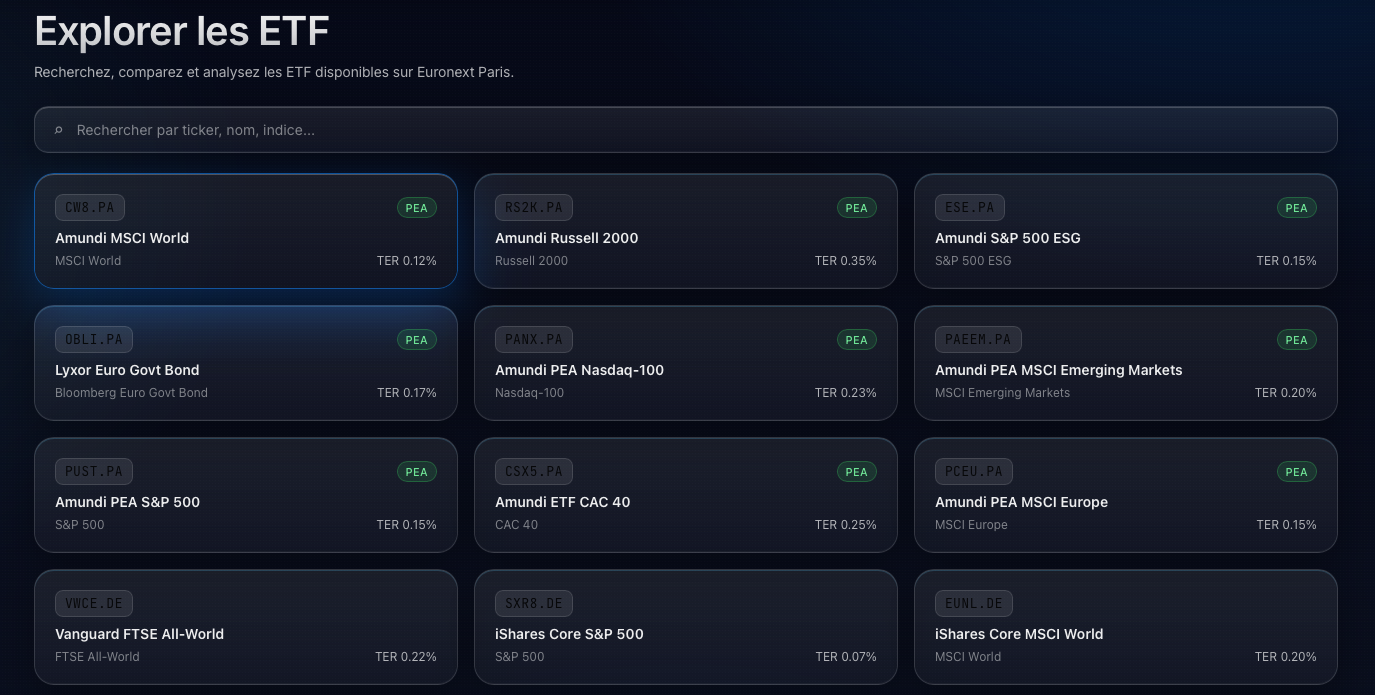
\includegraphics[width=0.95\linewidth]{img/ficheETF1.png}
\caption{Module A --- Liste des ETF disponibles sur Euronext Paris.}
\end{figure}

\begin{figure}[h]
\centering
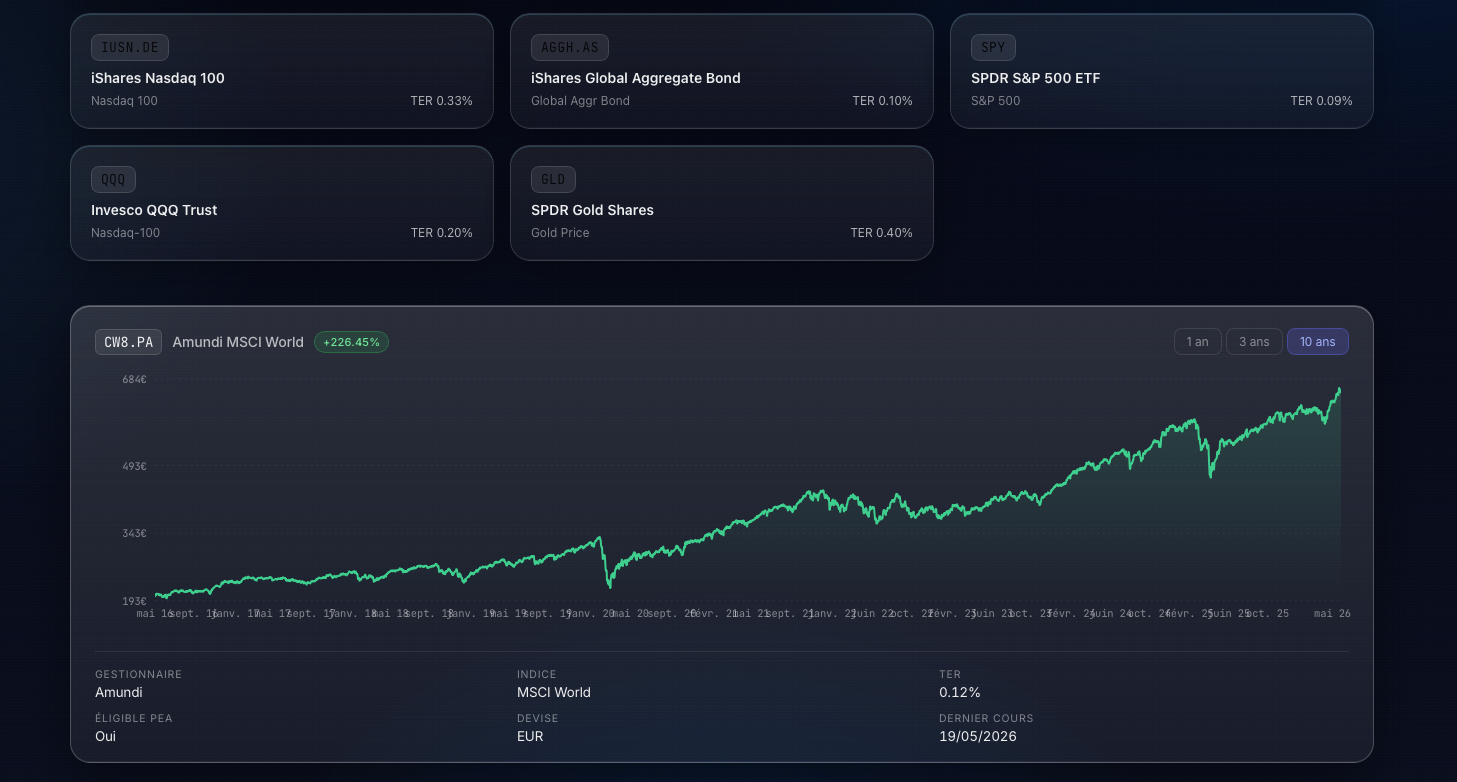
\includegraphics[width=0.95\linewidth]{img/ficheETF2.png}
\caption{Module A --- Fiche détaillée CW8.PA avec graphique de cours historique.}
\end{figure}

\begin{figure}[h]
\centering
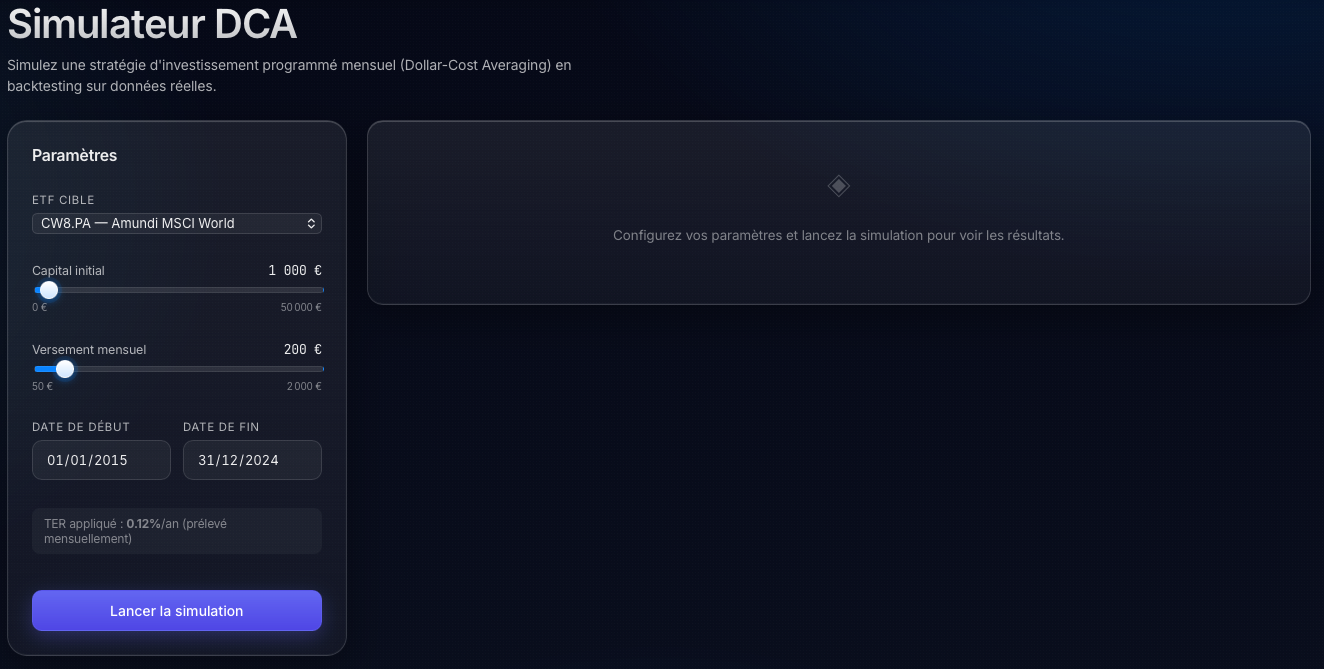
\includegraphics[width=0.95\linewidth]{img/simulateurDCA_av.png}
\caption{Module B --- Formulaire de paramétrage de la simulation DCA.}
\end{figure}

\begin{figure}[h]
\centering
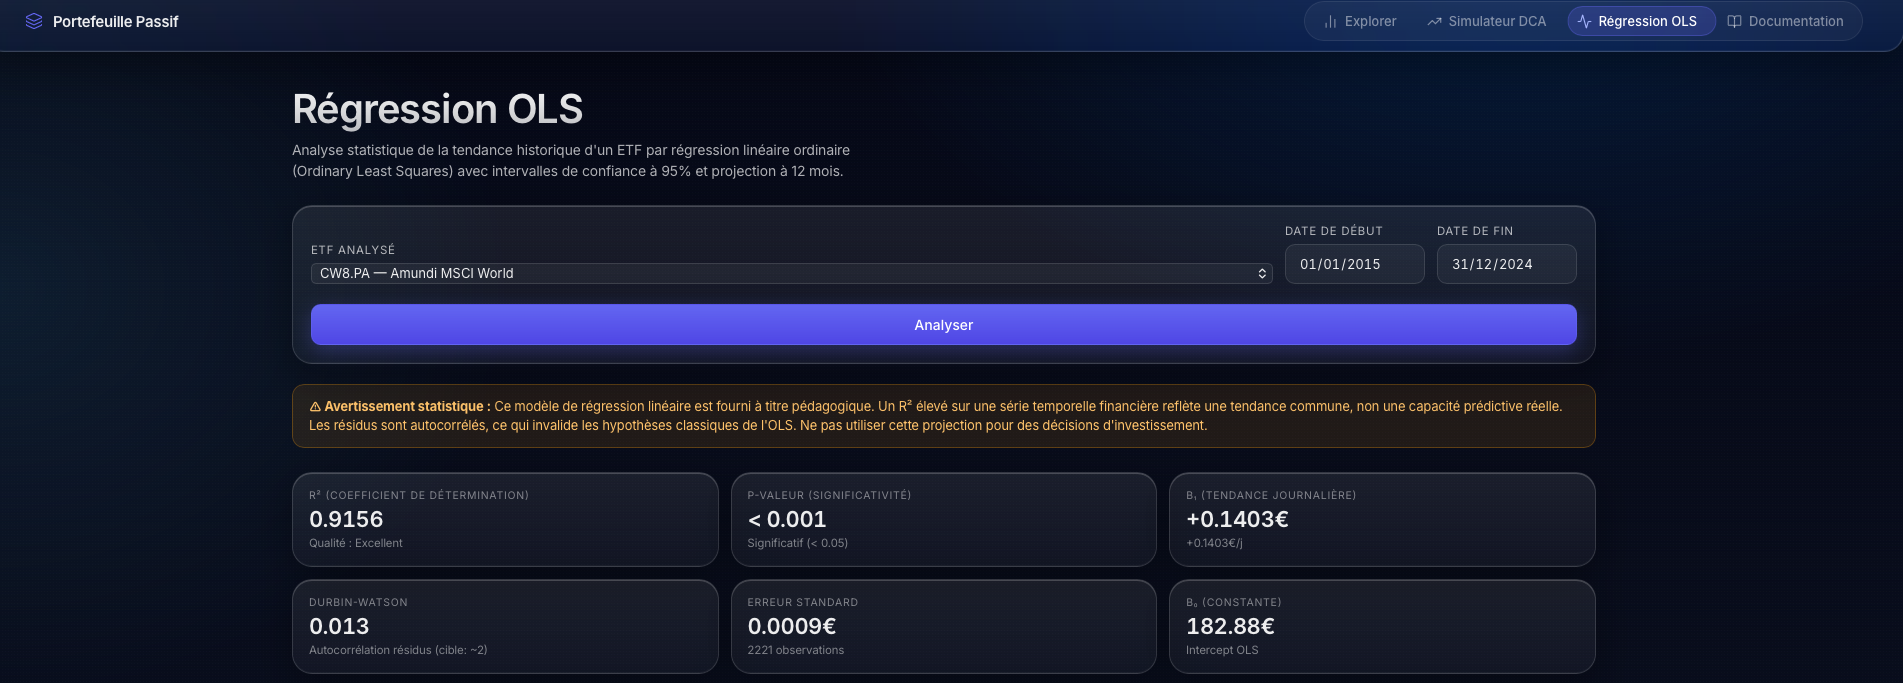
\includegraphics[width=0.95\linewidth]{img/regression1.png}
\caption{Module C --- Métriques de la régression OLS (R², Durbin-Watson, $\beta_0$, $\beta_1$).}
\end{figure}

\end{document}